% Autore= Enrico Salmaso

\subsubsection{UCS 7 - Monitoraggio degli accessi effettuati}
\begin{figure}[h]
	\centering
	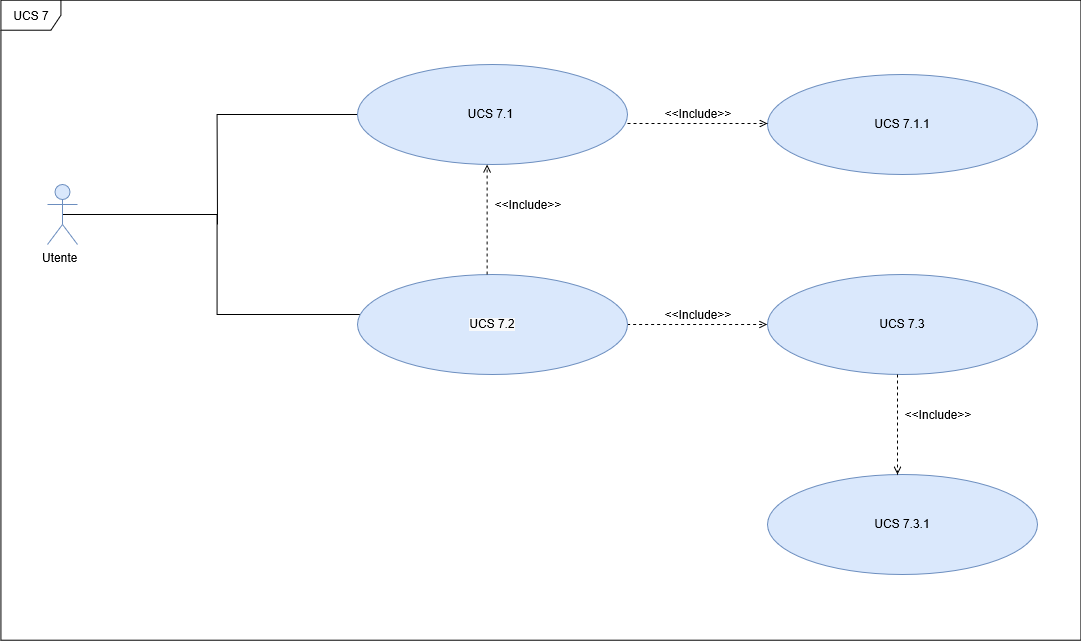
\includegraphics[scale=0.4]{sezioni/UseCase/Immagini/UCS7.png}
	\caption{UCS 7 - Monitoraggio degli accessi effettuati}
\end{figure}

\begin{itemize}
\item \textbf{Attori primari:} Amministratore autenticato
\item \textbf{Precondizione:} L'amministratore dispone di almeno un'organizzazione.
\item \textbf{Postcondizione:} L'amministratore ha monitorato gli accessi effettuati dagli utenti riconosciuti.
\item \textbf{Scenario principale:} L'amministratore, dopo aver selezionato l'organizzazione, accede alla funzionalità di visualizzazione della lista degli accessi per monitorare gli utenti.
\item \textbf{Flusso di eventi:} 
\begin{enumerate}
	\item L'amministratore ha selezionato l'organizzazione [UCS 3];
	\item L'amministrazione seleziona la funzionalità di visualizzazione della lista degli accessi;
	\item L'amministrazione può visualizzare gli accessi effettuati da un utente riconosciuto presso l'organizzazione [UCS 7.1] o in un luogo\ap{G} all'interno di essa [UCS 7.2];
\end{enumerate}
\end{itemize}

\subsubsection{UCS 7.1 - Visualizzazione degli accessi effettuati da un utente riconosciuto presso l'organizzazione}
\begin{itemize}
	\item \textbf{Attori primari:} Amministratore autenticato
	\item \textbf{Precondizione:} L'amministratore ha effettuato l'accesso alla funzionalità di monitoraggio degli accessi effettuati.
	\item \textbf{Postcondizione:} L'amministratore ha visualizzato la lista con gli accessi di un utente riconosciuto presso l'organizzazione.
	\item \textbf{Scenario principale:} L'amministratore esegue la procedura per visualizzare lo storico degli accessi effettuati presso l'organizzazione desiderata da un utente riconosciuto.
	L'amministratore può selezionare un luogo all'interno dell'organizzazione per monitorare gli accessi dell'utente al suo interno[UCS 7.2].
	\item \textbf{Flusso di eventi:}
	\begin{enumerate}
	\item L'amministratore seleziona un utente preciso da una lista contente tutti i utenti riconosciuti dell'organizzazione;
	\item L'amministratore visualizza una lista con tutti gli accessi effettuati dall'utente selezionato presso l'organizzazione;
	\item L'amministratore ha la possibilità di ordinare gli accessi dell'utente all'organizzazione [UCS 7.1.1] [UCS 7.1.2] oppure di effettuare una ricerca tra di essi per gli accessi di uno specifico giorno [UCS 7.1.3].
	\end{enumerate}
\end{itemize}

\subsubsection{UCS 7.1.1 - Ordinamento per data decrescente della lista degli accessi}
\begin{itemize}
	\item \textbf{Attori primari:} Amministratore autenticato
	\item \textbf{Precondizione:} L'amministratore sta visualizzando lo storico accessi di un utente riconosciuto.
	\item \textbf{Postcondizione:} L'amministratore ottiene la lista di accessi riordinata per data in ordine decrescente.
	\item \textbf{Flusso di eventi:}
	\begin{enumerate}
		\item L'amministratore seleziona la funzionalità per riordinare lo storico degli accessi effettuati dall'utente riconosciuto per data in ordine decrescente.
	\end{enumerate}   
\end{itemize}

\subsubsection{UCS 7.1.2 - Ordinamento per data crescente della lista degli accessi}
\begin{itemize}
	\item \textbf{Attori primari:} Amministratore autenticato
	\item \textbf{Precondizione:} L'amministratore sta visualizzando lo storico accessi di un utente riconosciuto.
	\item \textbf{Postcondizione:} L'amministratore ottiene la lista degli accessi riordinata per data in ordine crescente.
	\item \textbf{Flusso di eventi:}
	\begin{enumerate}
		\item L'amministratore seleziona la funzionalità per riordinare lo storico degli accessi effettuati dall'utente riconosciuto per data in ordine crescente.
	\end{enumerate}
\end{itemize}

\subsubsection{UCS 7.1.3 - Ricerca degli accessi effettuati da un utente riconosciuto in un giorno specifico}
\begin{itemize}
	\item \textbf{Attori primari:} Amministratore autenticato
	\item \textbf{Precondizione:} L'amministratore sta visualizzando lo storico accessi di un utente riconosciuto.
	\item \textbf{Postcondizione:} L'amministratore ottiene la lista di accessi effettuati nel giorno selezionato.
	\item \textbf{Flusso di eventi:}
	\begin{enumerate}
		\item L'amministratore seleziona la funzionalità per visualizzare solo gli accessi avvenuti in un giorno specifico presso l'organizzazione;
		\item L'amministratore seleziona il giorno desiderato.
	\end{enumerate}  
\end{itemize}


\subsubsection{UCS 7.2 - Visualizzazione degli accessi effettuati da un utente riconosciuto presso un luogo all'interno dell'organizzazione}
\begin{itemize}
	\item \textbf{Attori primari:} Amministratore autenticato
	\item \textbf{Precondizione:} L'amministratore ha effettuato l'accesso alla funzionalità di monitoraggio degli accessi effettuati.
	\item \textbf{Postcondizione:} L'amministratore ha visualizzato la lista con gli accessi di un utente riconosciuto presso un luogo all'interno dell'organizzazione.
	\item \textbf{Scenario principale:} L'amministratore esegue la procedura per visualizzare lo storico degli accessi effettuati presso un luogo all'interno dell'organizzazione desiderata da un utente riconosciuto.
	\item \textbf{Flusso di eventi:}
	\begin{enumerate}
	\item L'amministratore seleziona un utente preciso da una lista contente tutti i utenti riconosciuti dell'organizzazione;
	\item L'amministratore seleziona un luogo all'interno dell'organizzazione;
	\item L'amministratore visualizza una lista con tutti gli accessi effettuati dall'utente selezionato presso un luogo all'interno dell'organizzazione;
	\item L'amministratore ha la possibilità di ordinare gli accessi dell'utente all'organizzazione [UCS 7.1.1] [UCS 7.1.2] oppure di effettuare una ricerca tra di essi per gli accessi di uno specifico giorno [UCS 7.1.3].
	\end{enumerate}
\end{itemize}




